In order to devise a simple model for golf ball flight we first must understand some
prerequisite physics for projectiles and fluid dynamics for the airflow over the ball. Understanding
how the fluid flows over the surface of the ball is crucial to understanding the difference between
the flight of a golf ball and that of a standard projectile. Quantifying this effect will be a large
component of this project.

There has been significant work done previously in understanding the fluid dynamics around a golf ball
and how a golf ball flies. We will attempt to review some of this literature in this chapter and summarise
previous work on the topic.

First though, we must understand how normal projectiles fly without taking into account fluid dynamics effects.
\section{Projectile Motion}
A projectile is a body fired into the air by an initial impulse and then allowed to fall back to ground under the
action of gravity alone. This is the most naive and simplistic model of golf ball flight, completely
ignoring all aerodynamic effects, however we must understand it before building up to a more
complex model.

Consider motion in a 2 dimensional plane, labelled by $x$ along the horizontal and $y$ along the vertical.
A projectile is given an initial speed of the form $\vv_0 = (v_x, v_y)$. We set the origin of the coordinate system to be the point at the start of the
trajectory, $(x_0, y_0) = (0,0)$. In this problem the acceleration on the projectile, after the initial
impulse, is constant and of the form
\begin{equation} \label{grav}
a_x = 0, \quad a_y = -g
\end{equation}
where $g$ is the acceleration due to gravity. Since the acceleration is constant we can use
the standard formulas for motion under constant acceleration to derive the dynamics of the
projectile \citet{yandf}, which are
\begin{subequations} \label{suvat}
\begin{align}
v &= v_0 + at \label{v} \\
x &= v_0 t + \frac{1}{2} a t^2 \label{xsuvat} \\
v^2 &= v_0^2 + 2ax \\
x &= \left(\frac{v_0 + v}{2}\right) t .
\end{align}
\end{subequations}
Where $v$ is the speed at a time $t$, $x$ is the distance from the origin of the coordinate system,
$a$ is the acceleration and $v_0$ is the initial speed.

We will write the equations in component form along the axes. Let $\vv_0$ be the initial velocity.
In component form these will be
\[
v_{0x} = v_0 \cos \alpha
\]
along the $x$-axis and
\[
v_{0y} = v_0 \sin \alpha
\]
where $v_0 = |\vv_0|$ and $\alpha$ is the angle $\vv_0$ makes with the $x$-axis. Now using \eqref{grav}
and \eqref{v} we may find
\begin{subequations} \label{proj-v}
\begin{align}
v_x &= v_0 \cos \alpha \\
\shortintertext{and}
v_y &= v_0 \sin \alpha - gt . \label{proj-vy}
\end{align}
\end{subequations}

Now, using \eqref{xsuvat} (or by integrating \eqref{proj-v} with respect to $t$), we can obtain the 
standard formulas for the $x$ and $y$ positions during the flight of the projectile:
\begin{subequations}
\begin{align}
x &= (v_0 \cos \alpha) t \label{proj-x} \\
\shortintertext{and}
y &= (v_0 \sin \alpha) t - \frac{1}{2} g t^2 \label{proj-y} .
\end{align}
\end{subequations}

Eliminating $t$ between these equations demonstrates that projectiles follow parabolic
paths, giving
\begin{equation}
y = x \tan \alpha - \frac{g}{2v_0^2 \cos^2 \alpha} x^2
\end{equation}
for the path of the projectile.

Finally we may use these equations to find the maximum height, range and time of flight for a
projectile. The maximum height is obtained when $v_y = 0$ and solving \eqref{proj-vy} with this
condition gives
\begin{equation} \label{proj-height}
t_{H} = \frac{v_0 \sin \alpha}{g} .
\end{equation}
The range is obtained by solving for $y=0$ in \eqref{proj-y} and selecting the non trivial root for $t$
of
\begin{equation}
t_{F} = \frac{2 v_0 \sin \alpha}{g}
\end{equation}
where $t_{F}$ is the time of flight for the projectile. Inserting this into \eqref{proj-x} gives
\[
x = \frac{2 v_0^2 \cos \alpha \sin \alpha}{g}
\]
and recalling that $\sin 2 \alpha = 2 \cos \alpha \sin \alpha$ gives
\begin{equation}
x = \frac{v_0^2 \sin 2 \alpha}{g}
\end{equation}
for the range of the projectile.
\subsection{3D Projectile Motion}

Projectile motion in 3 dimensions works in exactly the same fashion as 2D projectile motion. Here we
will take the $z$-axis to be the vertical and $x$ and $y$ axes to be labelling the surface. The only
component of acceleration is along the $z$-axis, with
\[
a_z = -g
\]
as before. All other equations remain the same.

\section{Basic Aerodynamics}

Of course, the flight of a golf ball is inevitably affected by aerodynamics. As such we need to have
some understanding of how aerodynamic effects will . In particular, we will need to understand how boundary layers
form on and separate from the surface of the golf ball and how this effects the drag on the ball.
First we will review some basic fluid mechanics.

\subsection{Fluid Mechanics}

In this project we will model the air flowing around the ball as being an incompressible fluid. This
is an Eulerian description of fluid flow, viewing the fluid as though the ball is fixed in the centre
of the coordinate system and the fluid moving around the ball \citet{Ruban2014}.

We will not concern ourselves with a full discussion of fluid mechanics from basic principles here, 
instead we will simply state some useful results predominantly following \citet{Ruban2014} and 
\citet{sears}.

Let $\vv$ be the fluid velocity, which is a function of the the position $\rvec$ from the origin of the
coordinate system and of time $t$. Let $\rho$ be the density of the fluid and $p$ the pressure. 
We define the material derivative to be (as a differential operator)
\begin{equation} \nonumber
\frac{D}{Dt} = \frac{\partial}{\partial t} + (\vv \cdot \nabla)
\end{equation}
and represents the rate of change of some quantity within the fluid, while moving with a small element
of the fluid flow. That is, in a description where the fluid moves relative to the coordinate system
the material derivative measures the rate of change as seen by a moving fluid element.

At all points within the fluid the mass continuity equation must apply
\begin{equation} \label{mass-cont}
\matdef{\rho} + \rho \nabla \cdot \vv = 0 .
\end{equation}
This equation encodes the condition that mass is conserved within a fluid without any sources or sinks.
In an incompressible fluid, as we will be primarily conserved with in this project, $\rho$ will not
change with time, and as such $D \rho / D t = 0$. As a consequence, both terms on the left hand side of
\eqref{mass-cont} must be zero everywhere within the fluid, and therefore the equation reduces to
\begin{equation} \label{incompress}
\nabla \cdot \vv = 0
\end{equation}
for an incompressible fluid.

The continuity equation gives one equation for the velocity components $u,v,w$\footnote{
	The convention within fluid mechanics is that the $x,y,z$ velocity components are called $u,v,w$
	respectively. That is \[
		v_x = u, \qquad v_y = v, \qquad v_z = w .
	\]
} within a fluid. In order to specify the pressure and velocity everywhere we therefore require three
more equations to determine the system. These three equations are supplied by considerations of
energy and momentum conservation. Keeping all of these in mind, we may write a
momentum equation in the form
\begin{equation} \label{momentum}
\rho \matdef{\vv} = - \nabla p + \mu \nabla^2 \vv + \ff
\end{equation}
where $\ff$ is body force per unit volume acting on the fluid (for example a gravitational force) 
and $\mu$ is the viscosity of the fluid.

Equations \eqref{incompress} and \eqref{momentum} when taken together form the Navier-Stokes equations
for the velocity and pressure fields within an incompressible fluid. It is well known that these
equations are highly non-linear and exceedingly difficult to solve both analytically and numerically,
except in special circumstances.

From solutions the Navier-Stokes equations emerges a number of fascinating effects within fluid 
dynamics. In this project, we are particularly interested in boundary layer effects and turbulence.

\subsection{Non Dimensional Variables and the Reynolds Number}

In physics we are often interested in understanding the behaviour of a system independent of a
choice of units \citet{0143-0807-31-4-019}. Instead, we wish to
have a system of measurement which does not depend intrinsically on one set on units, but on more 
fundamental ideas such as length or mass. We desire this for two main reasons:
\begin{itemize}
	\item Physical statements should not have any dependency on the units they are stated in.
	Non-dimensionalising the problem ensures that this is the case.
	\item Using non-dimensional variables allow problems of different scales to be compared to each 
	other on an equal footing. Often the points when the physical behaviour of the system changes 
	will depend on some non-dimensional parameter, as we will see with turbulence later \citet{jensen2013introducing}.
\end{itemize}

Additionally, analysing the fundamental dimensions of a physical problem can yield information on the
functional form of quantities within the model without having to use more advanced mathematical
techniques to derive such results. By simply understanding the dependency on fundamental units we
often can find interesting scaling laws for functions of interest.

The fundamental dimensions (only those which will be useful in this project) are as follows:
\begin{table}[h]
\centering
\begin{tabular}{l c}
Dimension & Symbol \\
\hline
Length & $L$ \\
Mass & $M$ \\
Time & $T$
\end{tabular}
\caption[List of fundamental dimensions]{List of fundamental dimensions we will require in this report.}
\end{table}

Any quantities of interest can be written using these variables: for example, an area $A$ would have 
the dimensions $[A] = L^2$ and a velocity $[V] = L/T$.

Physical laws can, in general, be written as \citet{0143-0807-31-4-019}
\begin{equation} \label{functional}
q_{0} = f(q_1,q_2,\ldots,q_n)
\end{equation}
where $q_0$ is a physical quantity we are interested in obtaining, $q_1,\ldots,q_n$ are independent
physical quantities and $f$ is a functional relationship between them.

When analysing the dimensions of a problem we must ensure that the following conditions are
satisfied
\begin{itemize}
\item Both sides of \eqref{functional} must have the same fundamental dimensions.
\item Any sum of $q_i$ must have the same dimensions.
\item Any function of $q_i$ (say, exponential or trigonometric) must be dimensionless. This is as a 
direct result of the last condition and being able to expand these functions as a power series.
\end{itemize}

We will demonstrate this technique in section~\ref{sec:drag}.

One of the aims of dimensional analysis is to find groupings of physical quantities which are
dimensionless. These have useful properties of scale invariance which leads to natural parameterisations
for physical problems.

Within fluid mechanics one such dimensionless grouping which manifests often is the Reynolds
number, defined as 
\begin{equation} \label{re-number}
Re = \frac{\rho \vv L}{\mu} .
\end{equation}
This quantity represents the ratio of inertial forces to viscous ones, and we will make considerable
use of it within the project. The Reynolds number, in some ways, can be considered to be a non
dimensional analogue of the velocity, taking into account the intrinsic length scale of the problem
under consideration.

\subsection{Boundary Layers}

One of the fundamental ideas within fluid mechanics is that of the no slip condition. The no slip 
condition specifies that when a fluid encounters a solid body it must, at the surface of the body,
take the velocity and temperature of that body. This means that there will be a thin layer of fluid
around the body where the velocity changes from that of the overall stream to match the velocity of
the solid body: this layer is referred to as the boundary layer.

The equations which govern the flow within the boundary layer are a simplified version of the
Navier-Stokes equations, taking into account the order of magnitude of the boundary layer compared to
the size of the body. The derivation of these equations completed by scaling the Navier-Stokes 
based on the assumption that the boundary layer is much smaller than the body size \citet{anderson}.

In 2D these equations look as follows:
\begin{subequations}
\begin{align}
\pd{u}{x} + \pd{v}{y} &= 0 &\text{(Continuity equation)} \\
u\pd{u}{x} + v\pd{u}{y} &= -\frac{1}{\rho} \pd{p}{x} +
\nu \spd{u}{y} &\text{($x$ momentum)} \\
\frac{1}{\rho} \pd{p}{y} &= 0 &\text{($y$ momentum)}
\end{align}
\end{subequations}
where $\nu$ is the kinematic viscosity, defined as $\nu = \mu / \rho$.

\subsection{Lift and Drag} \label{sec:drag}

In order to go beyond modelling golf ball flight as simply that of a projectile we must understand 
how the lift and drag forces affect the flight of the ball. We can use dimensional analysis arguments
to obtain a functional form for these effects. Here we follow the analysis of 
\citet{jensen2013introducing} in order to demonstrate the analysis for the drag force. The lift is
found in a similar way.

One first must ask what physical terms we would expect the drag to have a dependency on. We would
expect some dependency on the velocity $v$ of the object through the fluid, on the shape of the body and
a characteristic length scale $r$ for the body, on the density of the fluid $\rho$, and finally on
the viscosity of the fluid $\nu$. As noted in \citet{jensen2013introducing} we have no dependency from
the mass of the body on the drag. As per the rest of this project we also assume the fluid is
incompressible.

Forming an equation in the style of \eqref{functional} between these quantities and the drag force 
$D$ we obtain
\begin{equation} \label{drag-dimensions}
D = g \, v^{\alpha} r^{\beta} \rho^{\gamma} \nu^{\delta}
\end{equation}
where $g$ is a dimensionless constant which will take into account the shape of the body and
potentially other dimensionless parameters such as the Reynolds number \eqref{re-number}.

We attempt to obtain values of $\alpha, \beta, \gamma, \delta$ which balances \eqref{drag-dimensions}.
The dimensions of the quantities in \eqref{drag-dimensions} are as follows:
\begin{equation} \nonumber
[D] = M L T^{-1}, \qquad [v] = L T^{-1}, \qquad [r] = L, \qquad [\rho] = M L^{-3}, \qquad [\nu] = M L^{-1} T^{-1}
\end{equation}
and so balancing \eqref{drag-dimensions} implies that
\begin{equation}
M L T^{-2} = M^{\gamma + \delta} L^{\alpha + \beta - 3\gamma - \delta} T^{-\alpha-\delta} .
\end{equation}

Equating the powers leads to a system of 3 linear equations in 4 variables for each fundamental unit
given by
\begin{subequations}
\begin{align}
1 &= \gamma + \delta \\
1 &= \alpha + \beta - 3 \gamma - \delta \\
-2 &= \alpha - \delta
\end{align}
\end{subequations}
for $M, L$ and $T$ respectively.

Using these equations we can eliminate all but one of the parameters, and writing all these in terms
of $\delta$ we can find
\begin{align}
D &= g v^{2-\delta} r^{2-\delta} \rho^{1-\delta} \nu^{\delta} \\
\shortintertext{and rearranging these powers}
D &= g \rho r^2 v^2 \left(\frac{\nu}{\rho r v}\right)^{\delta} .
\end{align}
We can then recognise that the term in the brackets is $1/Re$. Following \citet{jensen2013introducing}
we can derive, using a similar analysis, that $g$ must also have some functional dependency on the
Reynolds number, and as such
\begin{equation} \label{drag-functional}
D = \rho r^2 v^2 f(Re) .
\end{equation}
The form of $f$ depends on the velocity of the body moving through the fluid. 

In the low velocity limits of low and high velocity we find slightly different forms for the dependence 
on velocity. In the low velocity limit, the dependency on velocity is only linear, that is
\begin{equation}
D = g \nu r v .
\end{equation}
where $g$ is simply related to the shape of the body. This is known as stokes drag, corresponding to
laminar flow about the body.
Whereas in the high velocity limit we would expect turbulent flow behind the body. This is the case
which manifests during the flight of a golf ball, and the distinction will be important later.
\begin{equation} \label{turb-drag}
D = g \rho r^2 v^2
\end{equation}

On comparison with \eqref{drag-functional} we see that at low velocity, $f(Re) \propto Re^{-1}$
and in the high velocity case $f(Re)$ is independent of $Re$.

Within the literature related to fluid dynamics and aerodynamics \eqref{turb-drag} is normally written
with different names for the variables, namely 
\begin{equation} \label{drag}
F_{D} = \frac{1}{2} \rho \vv^2 A c_{D}
\end{equation}
where $F_{D}$ is the drag force, and $c_{D}$ is the dimensionless drag coefficient. Is it this form
we will use from here on. 

An expression for the lift can be derived using very similar analysis, and has the same form as the
drag:
\begin{equation} \label{lift}
F_{L} = \frac{1}{2} \rho \vv^2 A c_{L}
\end{equation}
where here $c_{L}$ is the lift coefficient.
\subsection{Boundary Layer Separation and the Magnus Effect}

\citet{Seifert2012,Kharlamov2007}

\begin{figure}[h]
\centering
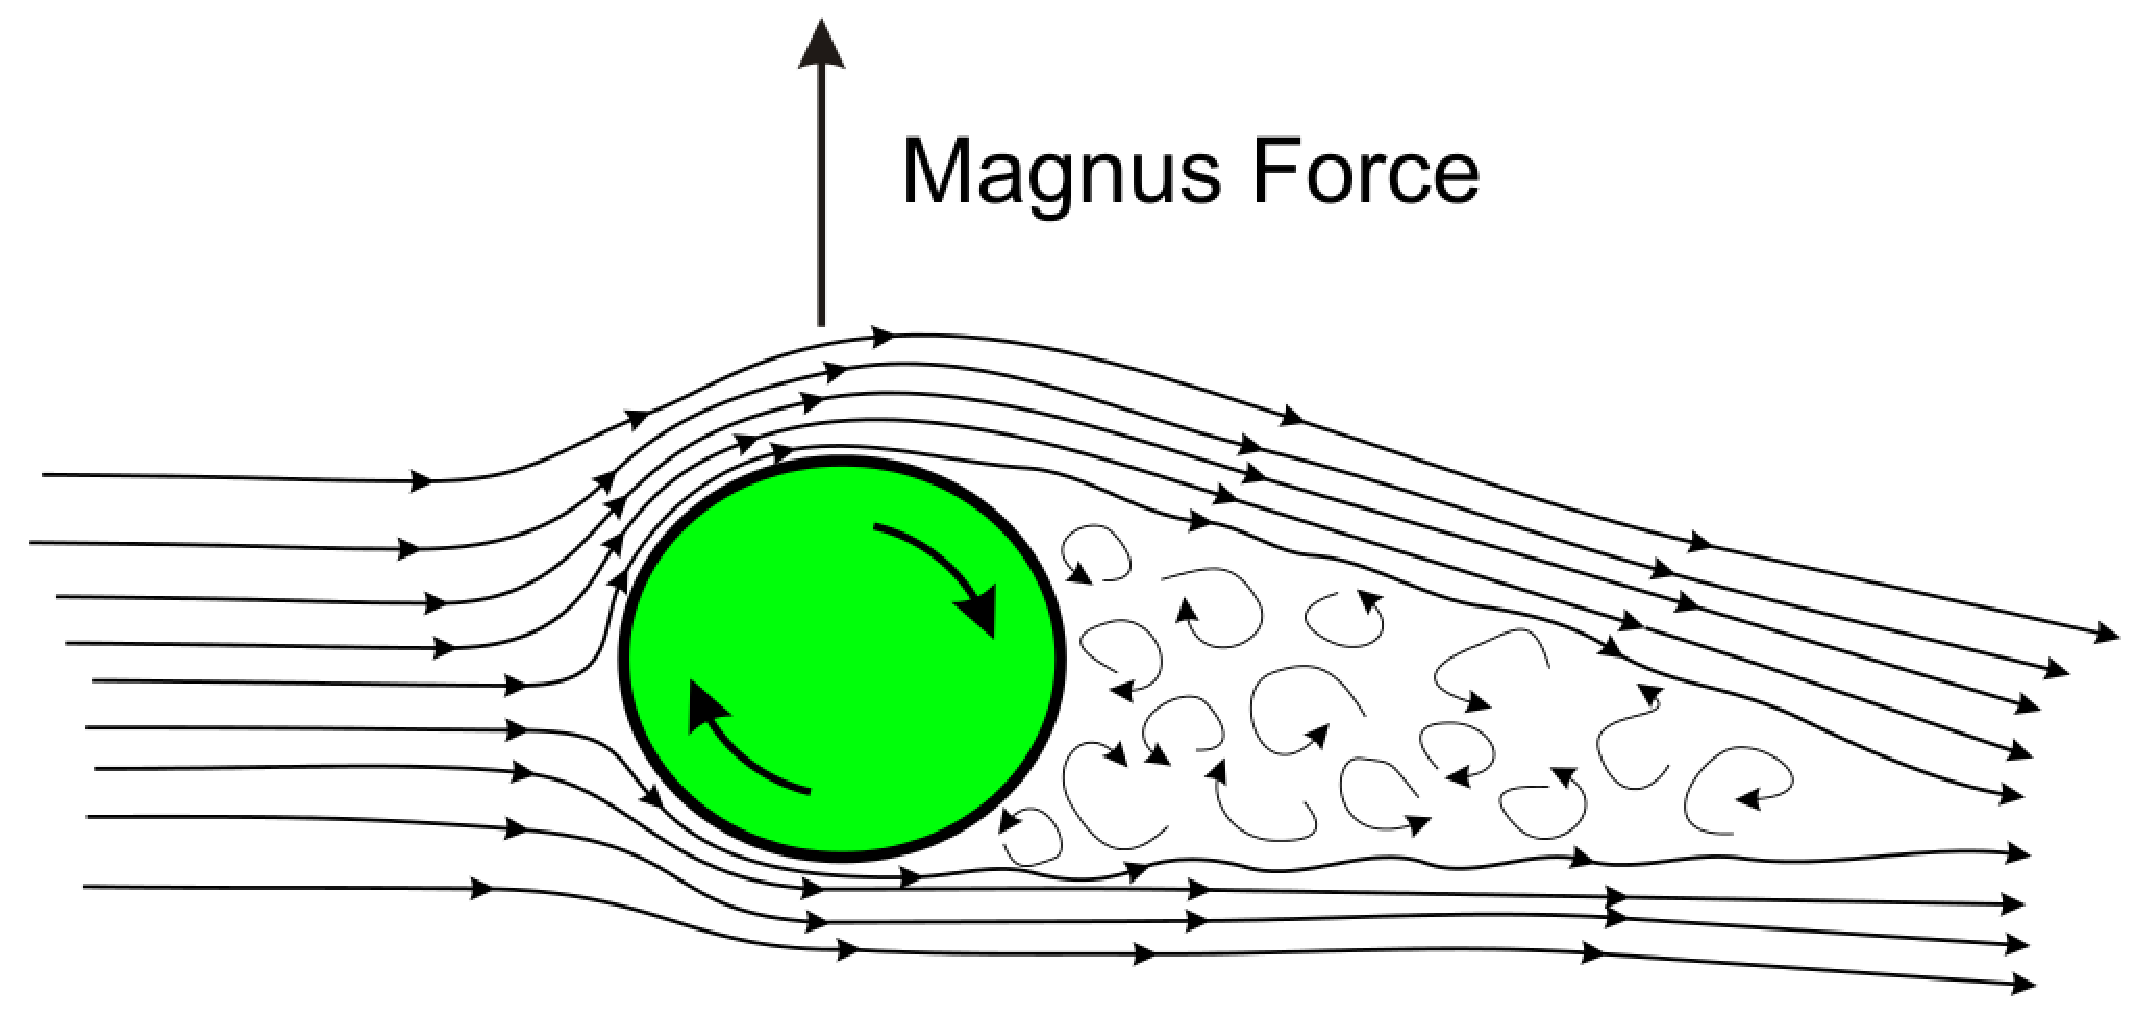
\includegraphics[scale=0.45]{../images/magnus.pdf}
\caption[A diagram of the Magnus effect]{A diagram of the Magnus force on a rotating sphere.
Adapted from \url{http://en.wikipedia.org/wiki/File:Sketch_of_Magnus_effect_with_streamlines_and_turbulent_wake.svg}.}
\end{figure}

\section{Previous Work on Modelling Golf Ball Flight}

There has been considerable attention within the scientific literature to modelling the flight of a
golf ball, both due to the considerably industry surrounding the game and the interesting fluid
dynamics which results from golf ball flight. A small selection of such papers are
\citet{Smits2004,Bearman1976,Penner2003,Alam2011,Kensrud2010,Leong2007} however there are many more
which could be discussed.

\subsection{Computational Simulations of Golf Ball Flight}

\citet{Smith2010,Beratlis2012Numerical}

\section{Measuring Golf Ball Trajectories}

\citet{Martin2012}